
\section{Additional Experimental Results}
%% \subsection{Bayesian Neural Network Regression}\label{section:gaussian_additional}
%% \begin{figure}
%%   \centering
%% %%   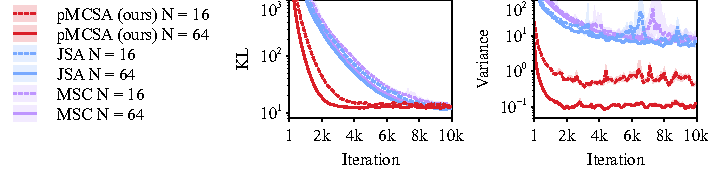
\includegraphics[scale=1.0]{figures/gaussian_02.pdf}
%%   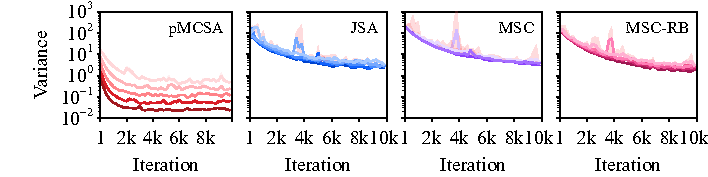
\includegraphics[scale=1.0]{figures/gaussian_04.pdf}
%%   \vspace{-0.08in}
%%   \caption{\textbf{Gradient variance versus iteration and computational budget (\(N\)).
%%       pMCSA not only achieves the least gradient variance, but its variance also scales better with \(N\).
%%     }
%%     The colors range from light (\(N=2^3\)) to dark (\(N=2^7\)) representing the computational budgets \(N \in [2^3, 2^4, 2^5, 2^6, 2^7]\).
%%     The target distribution is a 100-D multivariate Gaussian with \(\nu = 500\).
%%     The error bands are the 80\% quantiles obtained from 8 replications.
%%   }
%% \end{figure}

\subsection{Bayesian Neural Network Regression}\label{section:bnn_additional}
\begin{figure}[ht]
  \centering
  \subfloat[\textsf{yacht}]{
    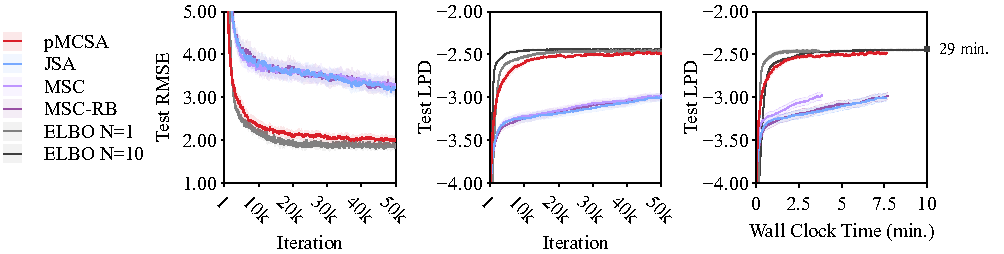
\includegraphics[scale=0.9]{figures/yacht_01.pdf}
    \vspace{-0.05in}
  }\vspace{0.05in}\\
  \subfloat[\textsf{concrete}]{
    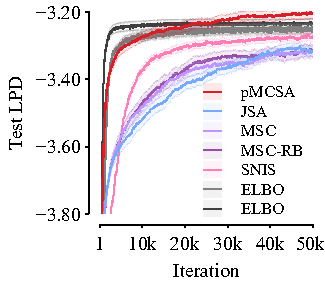
\includegraphics[scale=0.9]{figures/concrete_01.pdf}
    \vspace{-0.05in}
  }\vspace{0.05in}\\
  \subfloat[\textsf{airfoil}]{
    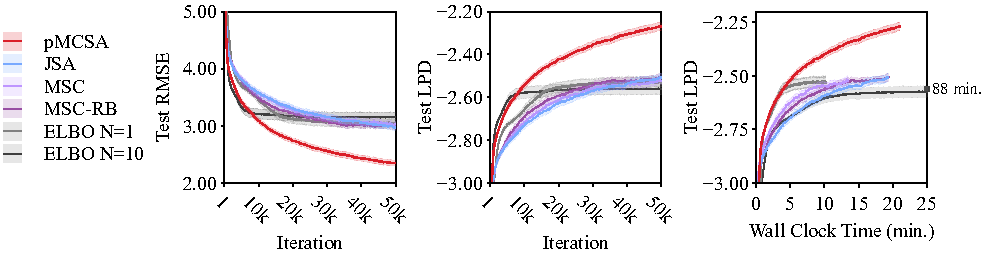
\includegraphics[scale=0.9]{figures/airfoil_01.pdf}
    \vspace{-0.05in}
  }\vspace{0.05in}\\
  \subfloat[\textsf{energy}]{
    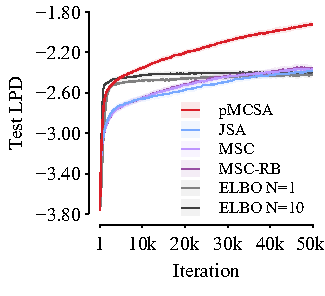
\includegraphics[scale=0.9]{figures/energy_01.pdf}
    \vspace{-0.05in}
  }
  \caption{\textbf{Test root-mean-square error (RMSE) and test log predictive density (LPD) on Bayesian neural network regression.} 
    The grey squares (\textcolor{darkgrey}{\(\blacksquare\)}) mark the performance of ELBO \(N=10\) at the wall clock time shown next to it.
  The error bands show the 95\% bootstrap confidence intervals obtained from 20 independent 90\% train-test splits.}
\end{figure}
%
\newpage
\begin{figure}[h]
  \centering
  \subfloat[\textsf{wine}]{
    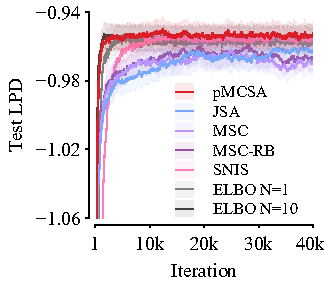
\includegraphics[scale=0.9]{figures/wine_01.pdf}
    \vspace{-0.05in}
  }\vspace{0.05in}\\
  \subfloat[\textsf{boston}]{
    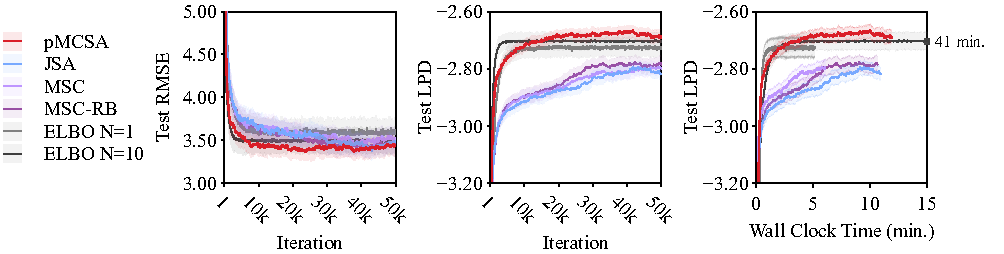
\includegraphics[scale=0.9]{figures/boston_01.pdf}
    \vspace{-0.05in}
  }\vspace{0.05in}\\
  \subfloat[\textsf{sml}]{
    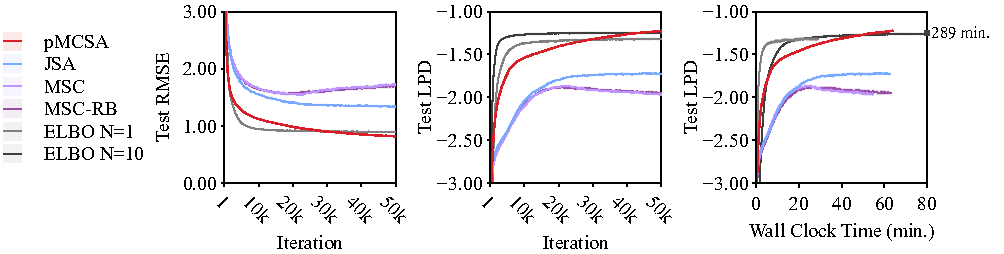
\includegraphics[scale=0.9]{figures/sml_01.pdf}
    \vspace{-0.05in}
  }\vspace{0.05in}\\
  \subfloat[\textsf{gas}]{
    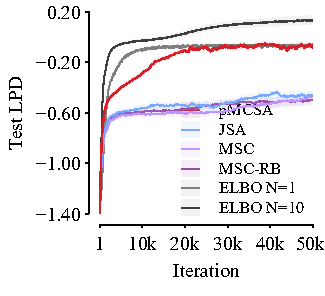
\includegraphics[scale=0.9]{figures/gas_01.pdf}
    \vspace{-0.05in}
  }
  \caption{\textbf{(continued) Test root-mean-square error (RMSE) and test log predictive density (LPD) on Bayesian neural network regression.}
    The grey squares (\textcolor{darkgrey}{\(\blacksquare\)}) mark the performance of ELBO \(N=10\) at the wall clock time shown next to it.
  The error bands show the 95\% bootstrap confidence intervals obtained from 20 independent 90\% train-test splits.}
\end{figure}

\newpage
\begin{figure}[H]
  \vspace{-0.10in}
  \centering
  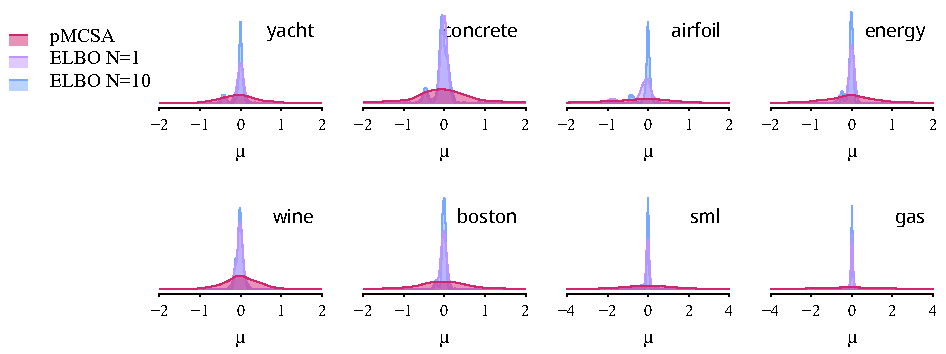
\includegraphics[scale=0.9]{figures/pruning_02.pdf}
  \vspace{-0.05in}
  \caption{\textbf{
      Distribution of the variational posterior mean of the BNN weights.
    }
    The density was estimated using a Gaussian kernel with Silverman's rule.
  }\label{fig:pruning_additional}
\end{figure}

\subsection{Robust Gaussian Process Regression}\label{section:gp_additional}
\begin{figure}[h]
  \centering
  \subfloat[\textsf{yacht}]{
    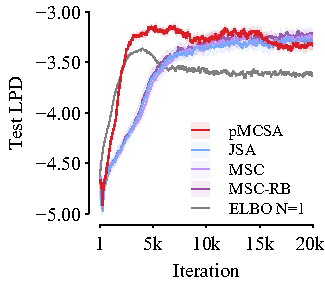
\includegraphics[scale=0.9]{figures/yacht_pgp_01.pdf}
    \vspace{-0.1in}
  }\vspace{0.05in}\\
  \subfloat[\textsf{airfoil}]{
    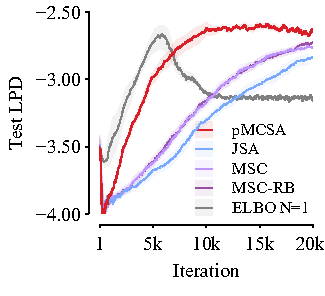
\includegraphics[scale=0.9]{figures/airfoil_pgp_01.pdf}
    \vspace{-0.1in}
  }\vspace{0.05in}\\
  \subfloat[\textsf{boston}]{
    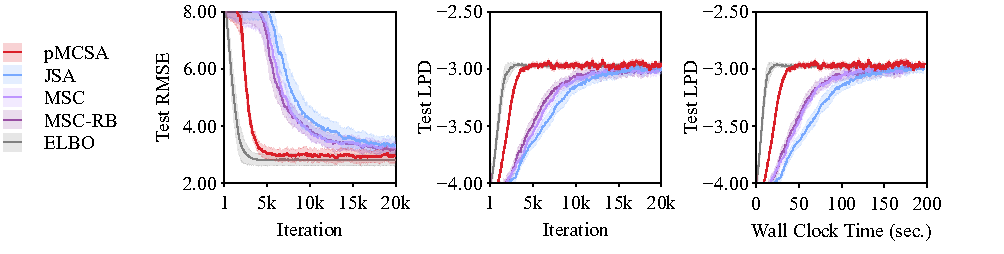
\includegraphics[scale=0.9]{figures/boston_pgp_01.pdf}
    \vspace{-0.1in}
  }\vspace{0.05in}\\
  \caption{\textbf{Test root-mean-square error (RMSE) and test log predictive density (LPD) on robust Gaussian process regression.}
  The error bands shows the 95\% bootstrap confidence interval obtained from 20 repetitions.}
\end{figure}
%
\newpage
\begin{figure}[ht]
  \subfloat[\textsf{energy}]{
    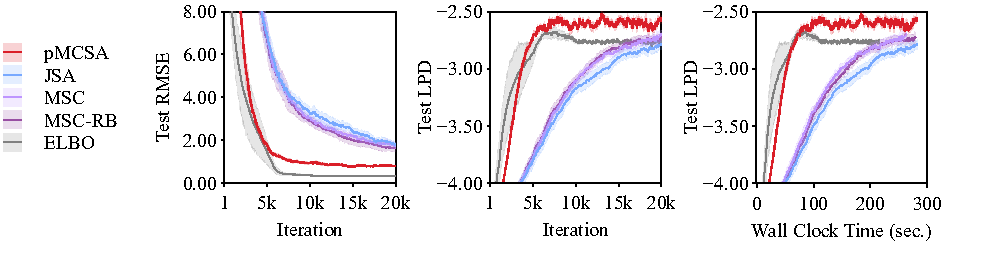
\includegraphics[scale=0.9]{figures/energy_pgp_01.pdf}
    \vspace{-0.1in}
  }\vspace{0.05in}\\ 
  \subfloat[\textsf{concrete}]{
    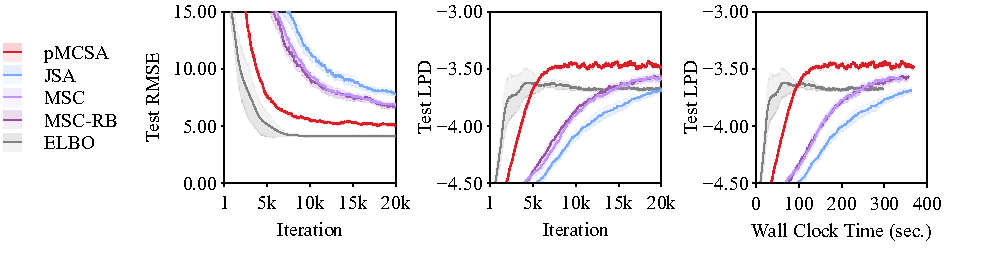
\includegraphics[scale=0.9]{figures/concrete_pgp_01.pdf}
    \vspace{-0.1in}
  }\vspace{0.05in}\\
  \subfloat[\textsf{wine}]{
    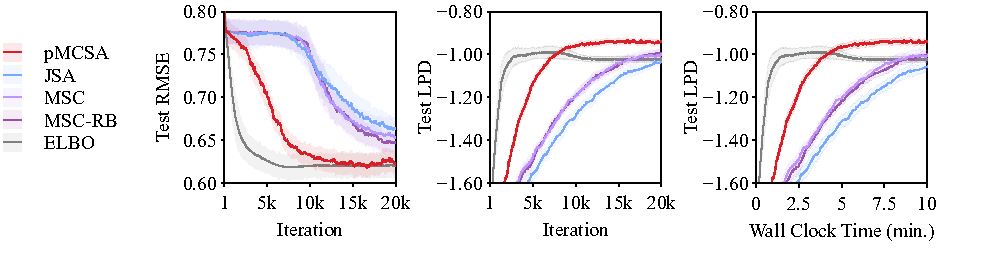
\includegraphics[scale=0.9]{figures/wine_pgp_01.pdf}
    \vspace{-0.1in}
  } \vspace{0.05in}\\
  \subfloat[\textsf{gas}]{
    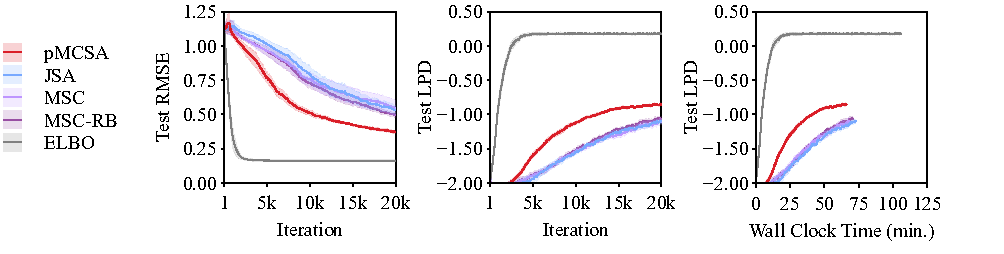
\includegraphics[scale=0.9]{figures/gas_pgp_01.pdf}
    \vspace{-0.1in}
  }
  \caption{\textbf{(continued) Test root-mean-square error (RMSE) and test log predictive density (LPD) on robust Gaussian process regression.}
  The error bands show the 95\% bootstrap confidence intervals obtained from 20 independent 90\% train-test splits.
  }
\end{figure}

%%% Local Variables:
%%% TeX-master: "master"
%%% End:
